% Document class and two-column conversion
\documentclass{report}
% dimensions of paper and relative text positioning
\usepackage[a4paper,top=2cm,bottom=2cm,left=2cm,right=2cm]{geometry}
% math symbols
\usepackage{amsmath}
\usepackage{amssymb}
% package for including URLs
\usepackage{url}
% Required for including images
\usepackage{graphicx}
\usepackage{float} % Required for specifying the exact location of a figure

% enable writing in greek
\usepackage[greek,english]{babel}
\usepackage[utf8]{inputenc}
%\usepackage[LGR]{fontenc}

\setlength{\parindent}{0pt} % Removes all indentation from paragraphs

% Start of the document
\begin{document}

% Set the language to greek
\selectlanguage{greek}

% Title page
\title{\Huge \bfseries Τεχνικές Βελτιστοποίησης \\ Τρίτο Παραδοτέο} %\Huge and \bfseries are used to make the title bigger and bold
\author{Παπαδάκης Κωνσταντίνος Φώτιος\vspace{0.5cm} \\  ΑΕΜ:10371} % \vspace{0.5cm} is used to add some vertical space between the author and the AEM
\date{\today}
% prints the title, author and date on a separate page
\maketitle

% Table of contents page
\tableofcontents

% General introduction
\chapter{Εισαγωγή}
\section{Ανάλυση Συνάρτησης $f(x_1,x_2)$}
Η συνάρτηση που θα εξετάσουμε στο τρίτο παραδοτέο είναι η εξής:
$$ f: \mathbb{R}^2 \to \mathbb{R},\; f(x_1,x_2) = \frac{1}{3} x_1^2 + 3x_2^2,\; x = [x_1 x_2]^T$$
Η μορφή της στον τρισδιάστατο χώρο είναι η εξής:
\begin{figure}[H]
    \centering
    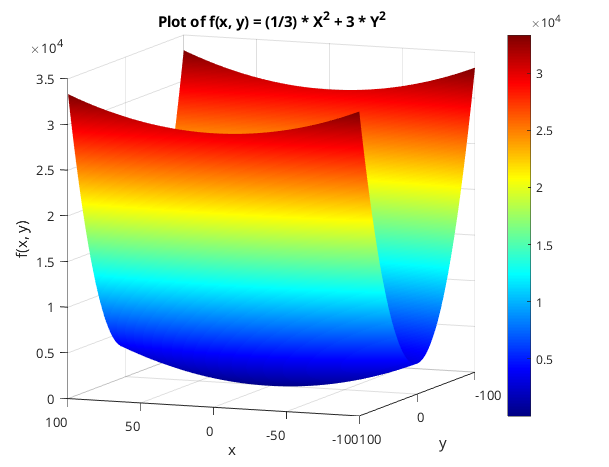
\includegraphics[width=0.5\textwidth]{media/visual.png}
    \caption{Οπτικοποίηση συνάρτησης $f(x,y)$}
\end{figure} 
Παρατηρούμε ότι η συνάρτηση σημειώνει ολικό ελάχιστο στο σημείο $(0,0)$.

% Steepest Descent: Various constant steps
\chapter{Θέμα 1}
\section{Εκφώνηση}
Να χρησιμοποιηθεί η Μέθοδος Μέγιστης Καθόδου (προηγούμενη εργασία) με ακρίβεια $\epsilon =
0.001$ και βήμα:
\begin{itemize}
    \item i) $\gamma_k$ = 0.1
    \item ii) $\gamma_k$ = 0.3
    \item iii) $\gamma_k$ = 3
    \item iv) $\gamma_k$ = 5
\end{itemize}
και οποιοδήποτε αρχικό σημείο εκκίνησης διαφορετικό του $(0,0)$. Τι παρατηρείτε
\selectlanguage{english};\selectlanguage{greek} Να αποδειχθούν τα αποτελέσματα αυτά 
με μαθηματική αυστηρότητα.
\section{Λύση}
Επέλεξα το σημείο εκκίνησης $(-10,-10)$ ως ένα σημείο αρκετά απομακρυσμένο από το ολικό ελάχιστο, 
κρίνοντας πάντα από την οπτικοποίηση της συνάρτησης μέσω \selectlanguage{english}Matlab.
\selectlanguage{greek}Έτσι θα μπορέσουμε να παρακολουθήσουμε καλύτερα την σύγκλιση του αλγορίθμου.
Το διάγραμμα που προκύπτει από την εκτέλεση του αλγορίθμου Μέγιστης Καθόδου με διάφορα σταθερά βήματα 
απέκρυπτε πληροφορία οπότε αποφάσισα να το σπάσω σε δύο επιμέρους διαγράμματα το καθένα με βήματα που
παρουσιάζουν παρόμοια συμπεριφορά:
\begin{itemize}
    \item Διάγραμμα που συγκλίνει στο ελάχιστο:
    \begin{figure}[H]
        \centering
        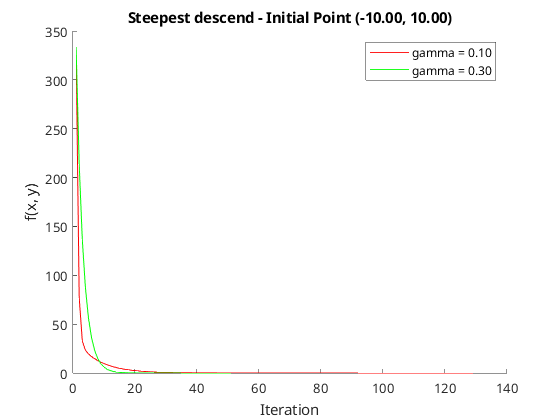
\includegraphics[width=0.7\textwidth]{media/thema1-1.png}
        \caption{Διάγραμμα Μέγιστης Καθόδου με σταθερά βήματα: 0.1, 0.3}
    \end{figure}
    \item Διάγραμμα που κάθε επανάληψη απομακρύνεται ολοένα και περισσότερο από το ελάχιστο:
    \begin{figure}[H]
        \centering
        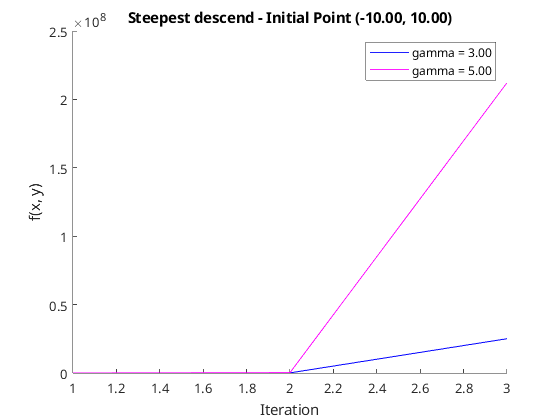
\includegraphics[width=0.7\textwidth]{media/thema1-2.png}
        \caption{Διάγραμμα Μέγιστης Καθόδου με σταθερά βήματα: 3, 5}
    \end{figure}
    Σε κάθε επανάληψη η απομάκρυνση που σημειώνεται είναι αρκετά μεγαλύτερη από αυτή της
    προηγούμενης επανάληψης έτσι ώστε η γραφική παράσταση της $f(x,y)$ μέχρι εκείνο το 
    σημείο να φαντάζει σαν να ταυτίζεται με τον άξονα $x'x$. 
    \begin{figure}[H]
        \centering
        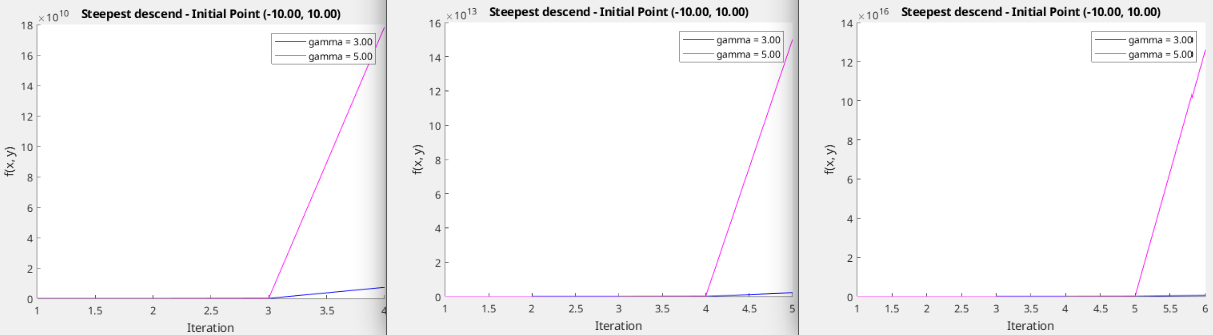
\includegraphics[width=0.8\textwidth]{media/thema1-2-2.png}
        \caption{Διάγραμμα Μέγιστης Καθόδου με σταθερά βήματα: 3, 5}
    \end{figure}
\end{itemize}

\subsection{Μαθηματική Απόδειξη}
Αναλυτικά έχουμε:
$$f(x) = \frac{1}{3} x_1^2 + 3x_2^2$$
\begin{center}
    και
\end{center}
$$\frac{\partial f}{\partial x_1} = \frac{2}{3}x_1$$
$$\frac{\partial f}{\partial x_2} = 6x_2$$
Η εξίσωση που μας δίνει την σύγκλιση είναι:
$$x_{k+1} = x_k - \gamma_k \nabla f(x_k)$$
Χρησιμοποιώντας πίνακες, έχουμε:
$$x_{k+1} = \begin{bmatrix} x_{1k} \\ x_{2k} \end{bmatrix} - \gamma_k \begin{bmatrix} \frac{2}{3}x_{1k} \\ 6x_{2k} \end{bmatrix}$$
$$x_{k+1} = \begin{bmatrix} x_{1k} - \frac{2}{3}\gamma_k x_{1k} \\ x_{2k} - 6\gamma_k x_{2k} \end{bmatrix}$$
$$x_{k+1} = \begin{bmatrix} (1 - \frac{2}{3}\gamma_k)x_{1k} \\ (1 - 6\gamma_k)x_{2k} \end{bmatrix}$$
$$x_{k+1} = \begin{bmatrix} 1 - \frac{2}{3}\gamma_k & 0 \\ 0 & 1 - 6\gamma_k \end{bmatrix} \begin{bmatrix} x_{1k} \\ x_{2k} \end{bmatrix}$$
$$x_{k+1} = M \cdot x_k$$

Για να πούμε ότι για να συγκλίνει ο αλγόριθμος πρέπει η απόλυτη τιμή των ιδιοτιμών του πίνακα M: 
$$M = \begin{bmatrix} 1 - \frac{2}{3}\gamma_k & 0 \\ 0 & 1 - 6\gamma_k \end{bmatrix}$$
να είναι μικρότερες του 1. Οπότε:
$$|\lambda_1|= 1 - \frac{2}{3}\gamma_k < 1$$
$$|\lambda_2| = 1 - 6\gamma_k < 1$$

Οι οποίες γίνονται:
$$0 < \gamma_k < 3$$
$$0 < \gamma_k < \frac{1}{3}$$
Έτσι συμπεραίνουμε ότι σωστά στο διάγραμμα παρατηρούμε σύγκλιση για τα βήματα 0.1 και 0.3 και 
απομάκρυνση για τα βήματα 3 και 5.

\subsection{Εισαγωγή Περιορισμών}
Θεωρήστε τώρα τους περιορισμούς:
$$-10 <= x_1 <= 5$$  
\begin{center}
    και
\end{center}
$$-8 <= x_2 <= 12$$

% Steepest Descent: Projection [1]
\chapter{Θέμα 2}
\section{Εκφώνηση}
Να χρησιμοποιηθεί η Μέθοδος Μέγιστης Καθόδου με Προβολή, με $s_k = 5$, $\gamma_k = 0.5$,
σημείο εκκίνησης το $(5, -5)$ και ακρίβεια $\epsilon = 0.01$. Τι παρατηρείτε σε σχέση με το 
Θέμα 1\selectlanguage{english};\selectlanguage{greek}

\section{Λύση}
Εδώ εισάγουμε στην αναφορά για πρώτη φορά την έννοια της προβολής. Ο κώδικας μας μένει σχεδόν ίδιος.
Σημεία διαφοροποίησης είναι τα παρακάτω:
\begin{itemize}
    \item Χρησιμοποιείται μια νέα συνάρτηση υπολογισμού του επόμενου σημείου κατά την σύγκλιση.
    $$x_{k+1} = x_k + \gamma_k (\overline{x_k} - x_k)$$
    \centerline{όπου}
    $$\overline{x} = x_k - s_k \nabla f(x_k)$$
    \item Όταν το $\overline{x}$ βγαίνει εκτός ορίων προδιαγράφουμε μια συμπεριφορά κατάλληλη έτσι ώστε 
    να μας επαναφέρει στο επιθυμητό διάστημα.
\end{itemize}
Η γραφική αναπαράσταση των αποτελεσμάτων παραθέτεται παρακάτω:
\begin{figure}[H]
    \centering
    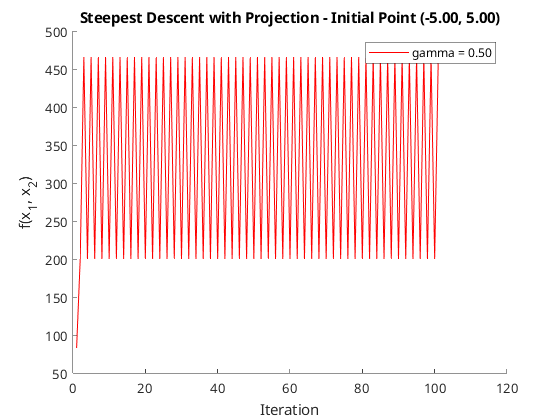
\includegraphics[width=0.7\textwidth]{media/thema2.png}
    \caption{Διάγραμμα Μέγιστης Καθόδου με προβολή $s_k = 5$, $\gamma_k = 0.5$}
\end{figure}
Ο αλγόριθμος δεν καταφέρνει να σταματήσει και καθ'όλη τη διάρκεια η συνάρτηση παίρνει τιμές από 
$f(x_1,x_2) = 5.33$ μέχρι $f(x_1,x_2) = 85.33$. Αποδείξαμε παραπάνω τον λόγο για τον οποίο η μέθοδος
μέγιστης καθόδου δεν συγκλίνει σε ελάχιστο. Βέβαια, στην προκειμένη περίπτωση το $\gamma_k$ δεν είναι
ο μόνος παράγοντας. Σίγουρα το $\gamma_k$ είναι μεγαλύτερο από το $\frac{1}{3}$ όμως όταν λαμβάνουμε 
υπόψιν το $s_k$, το οποίο είναι ο δεύτερος μας παράγοντας, συνειδητοποιούμε ότι είναι και αυτό πολύ 
μεγάλο έτσι ώστε να βοηθήσει το $\gamma_k$ να συγκλίνει. Εν τέλει, οδηγούμαστε σε μία συνεχή ταλάντωση 
όπου το βήμα του αλγορίθμου είναι πολύ μεγάλο για να υπάρχει οποιαδήποτε ουσιώδης προσέγγιση του ελαχίστου. 

% Steepest Descent: Projection [2]
\chapter{Θέμα 3}
\section{Εκφώνηση}
Να χρησιμοποιηθεί η Μέθοδος Μέγιστης Καθόδου με Προβολή, με $s_k = 15$, $\gamma_k = 0.1$,
σημείο εκκίνησης το $(-5,10)$ και ακρίβεια $\epsilon = 0.01$. Τι παρατηρείτε σε σχέση με τα Θέματα 1 
και 2\selectlanguage{english};\selectlanguage{greek} Προτείνετε έναν απλό πρακτικό τρόπο ώστε η 
μέθοδος να συγκλίνει στο ελάχιστο.

\section{Λύση}
Η γραφική αναπαράσταση των αποτελεσμάτων παραθέτεται παρακάτω:
\begin{figure}[H]
    \centering
    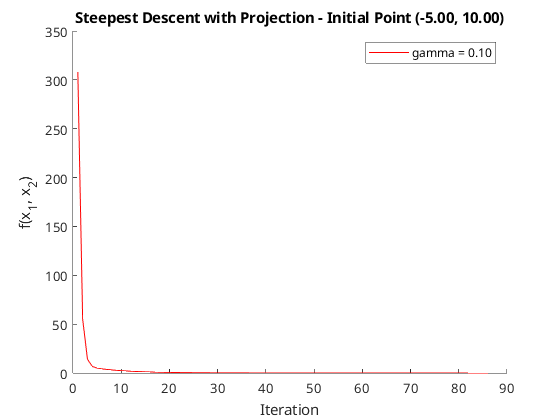
\includegraphics[width=0.7\textwidth]{media/thema3.png}
    \caption{Διάγραμμα Μέγιστης Καθόδου με προβολή $s_k = 15$, $\gamma_k = 0.1$}
\end{figure}
Για ακόμη μία φορά ο αλγόριθμος αδυνατεί να συγκλίνει ενώ κυμαίνεται περίπου μεταξύ των $f(x_1,x_2) = 0.04$ και
$f(x_1,x_2) = 3.241$. Για να συγκλίνει η μέθοδος μας στο ελάχιστο μπορούμε να κάνουμε μία από τις δύο παρακάτω
αλλαγές. Μπορούμε να μειώσουμε το $s_k$ ή το $\gamma_k$ έτσι ώστε να έχουμε μία πιο ομαλή σύγκλιση. Και στις δύο
περιπτώσεις όταν δεν βγαίνουμε εκτός ορίων η μείωση του ενός ισούται με τη μείωση του γινομένου τους που
είναι ουσιαστικά το νέο μας βήμα.
$$x_{k+1} = x_k + \gamma_k (\overline{x_k} - x_k)$$
$$x_{k+1} = x_k + \gamma_k (x_k - s_k \nabla f(x_k) - x_k)$$
$$x_{k+1} = x_k - \gamma_k * s_k \nabla f(x_k)$$

% Steepest Descent: Projection [3]
\chapter{Θέμα 4}
\section{Εκφώνηση}
Να χρησιμοποιηθεί η Μέθοδος Μέγιστης Καθόδου με Προβολή, με $s_k = 0.1$, $\gamma_k = 0.2$,
σημείο εκκίνησης το $(8, -10)$ και ακρίβεια $\epsilon = 0.01$. Σε αυτή την περίπτωση, έχουμε εκ των
προτέρων κάποια πληροφορία σχετικά με την σύγκλιση του αλγορίθμου\selectlanguage{english};
\selectlanguage{greek}Να γίνει η εκτέλεση του αλγορίθμου. Τι παρατηρείτε
\selectlanguage{english};\selectlanguage{greek}

\section{Λύση}
Η γραφική αναπαράσταση των αποτελεσμάτων παραθέτεται παρακάτω:
\begin{figure}[H]
    \centering
    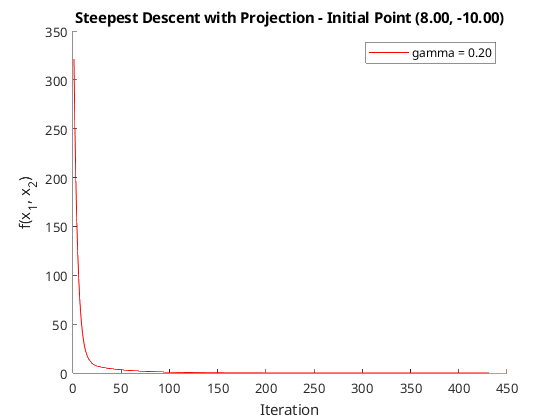
\includegraphics[width=0.7\textwidth]{media/thema4.png}
    \caption{Διάγραμμα Μέγιστης Καθόδου με προβολή $s_k = 0.1$, $\gamma_k = 0.2$} 
\end{figure}
Το ακριβές σημείο που σταμάτησε ο αλγόριθμος ήταν το $f(0.0149, 0) = 0.000074$ έπειτα από
$448$ επαναλήψεις. Εξαρχής μπορούσαμε να συμπεράνουμε ότι θα εμφάνιζε σύγκλιση στο ελάχιστο
αφού το $\gamma_k$ και το $s_k$ είναι ικανά μικρά για να αποφευχθεί η ταλάντωση που παρατηρήσαμε 
στα προηγούμενα θέματα 2, 3.

% End of the document
\end{document}